
\documentclass[aspectratio=169,10pt]{beamer}

\usetheme{Madrid}
\usecolortheme{default}

\usepackage{amsmath}
\usepackage{booktabs}
\usepackage{tikz}
\usepackage{pdfpcnotes}
\usetikzlibrary{arrows.meta,positioning}

% pdfpc speaker notes:
% \pnote{...} embeds notes in the PDF.

\setbeamertemplate{navigation symbols}{}
\setbeamertemplate{footline}[frame number]

\title[Weekly Progress]{
Exploring Reliable LLM Agent Swarms
}
\subtitle{Weekly Research Progress}
\author{Your Name}
\institute{Graduate Research Meeting}
\date{October 15, 2026}

\begin{document}

%========================================
% Slide 1: Title
%========================================
\begin{frame}
\titlepage

\pnote{
Today, I will present my weekly research progress.

My research focus is distributed systems
and their connection to multi-agent LLM systems.

This week, I investigated LLM agent swarms,
especially decentralized coordination
and reliability under communication failures.
}
\end{frame}

%========================================
% Slide 2: Previous Meeting
%========================================
\begin{frame}{Last Week and Feedback}

\textbf{Previous Focus}
\begin{itemize}
    \item Byzantine agreement for LLM agents
    \item Reliable multi-agent coordination
\end{itemize}

\vspace{0.5cm}

\textbf{Key Questions}
\begin{itemize}
    \item Why is distributed agreement necessary?
    \item Can existing mechanisms solve the problem?
    \item What makes LLM agents different?
\end{itemize}

\pnote{
Last week, I explored Byzantine agreement
for multi-agent LLM systems.

An important concern was whether distributed
agreement is actually necessary.

For example, simple browser coordination
may be handled by existing mutual exclusion.

Based on this discussion,
I reconsidered the research direction
and started investigating decentralized
LLM agent swarms.
}
\end{frame}

%========================================
% Slide 3: Background and Motivation
%========================================
\begin{frame}{Background and Motivation}

\begin{center}
\Large
\[
\boxed{\text{LLM Agents}}
+
\boxed{\text{Local Information}}
\]

\vspace{0.35cm}

\[
\Downarrow
\]

\vspace{0.35cm}

\[
\boxed{\text{Decentralized Coordination}}
\]
\end{center}

\vspace{0.4cm}

\begin{block}{Research Motivation}
How can autonomous agents coordinate
reliably without global information?
\end{block}

\pnote{
In decentralized agent systems,
each agent may have only local information.

Agents need to cooperate through
limited communication.

However, LLM agents can make incorrect
decisions and may fail to coordinate.

I want to understand how distributed
systems techniques can improve
their reliability.
}
\end{frame}

%========================================
% Slide 4: Related Work
%========================================
\begin{frame}{Related Work and Research Position}

\small
\begin{tabular}{p{3.1cm}p{4.1cm}p{4.1cm}}
\toprule
\textbf{Research} &
\textbf{Main Focus} &
\textbf{Perspective} \\
\midrule

Lamport et al. (1982)
& Byzantine Agreement
& Agreement guarantees \\

\addlinespace

Bonnet et al. (2014)
& Mobile Byzantine faults
& Agreement maintenance \\

\addlinespace

Cemri et al. (2025)
& Multi-agent failures
& Failure analysis \\

\addlinespace

Huang et al. (2025)
& Faulty LLM agents
& Collaboration resilience \\

\addlinespace

SwarmBench (2025)
& LLM swarm intelligence
& Local coordination \\

\bottomrule
\end{tabular}

\vspace{0.4cm}

\begin{block}{Research Position}
Distributed fault tolerance
$\times$ LLM swarm coordination
\end{block}

\pnote{
I reviewed research from two main areas.

The first is classical distributed systems,
including Byzantine agreement
and mobile Byzantine faults.

The second is multi-agent LLM research,
including failure analysis
and decentralized coordination.

SwarmBench is particularly relevant
because it studies agents with local
observations and communication.

My current interest is the intersection
of swarm coordination and fault tolerance.
}
\end{frame}

%========================================
% Slide 5: System Model
%========================================
\begin{frame}{SwarmBench: System Model}

\begin{center}
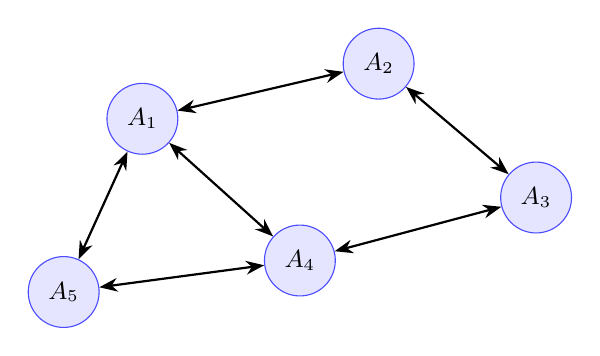
\begin{tikzpicture}[
agent/.style={
circle,draw=blue!70,fill=blue!10,
minimum size=0.9cm,font=\small
},
>=Stealth
]

\node[agent] (a) at (0,1.8) {$A_1$};
\node[agent] (b) at (3,2.5) {$A_2$};
\node[agent] (c) at (5,0.8) {$A_3$};
\node[agent] (d) at (2,0) {$A_4$};
\node[agent] (e) at (-1,-0.4) {$A_5$};

\draw[<->,thick] (a)--(b);
\draw[<->,thick] (b)--(c);
\draw[<->,thick] (a)--(d);
\draw[<->,thick] (d)--(c);
\draw[<->,thick] (a)--(e);
\draw[<->,thick] (d)--(e);

\end{tikzpicture}
\end{center}

\vspace{0.3cm}

\begin{itemize}
    \item Local observations
    \item Neighbor-to-neighbor communication
    \item Independent LLM-based decisions
\end{itemize}

\pnote{
SwarmBench evaluates LLM agents
in a decentralized environment.

Each agent observes only part
of the environment.

Agents communicate with nearby agents
and independently decide their actions.

The benchmark includes tasks such as
pursuit, synchronization, foraging,
flocking, and cooperative transport.

This provides a useful model
for studying distributed coordination.
}
\end{frame}

%========================================
% Slide 6: Existing Experimental Method
%========================================
\begin{frame}{SwarmBench: Experimental Method}

\begin{center}
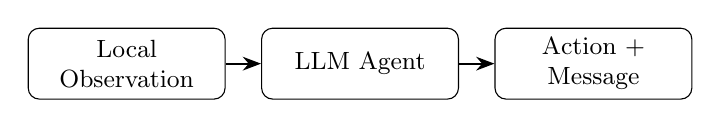
\begin{tikzpicture}[
box/.style={
draw,rounded corners,
minimum width=2.5cm,
minimum height=0.9cm,
align=center,font=\small
},
>=Stealth,
node distance=0.45cm
]

\node[box] (obs) {Local\\Observation};
\node[box,right=of obs] (llm) {LLM Agent};
\node[box,right=of llm] (act) {Action +\\Message};

\draw[->,thick] (obs)--(llm);
\draw[->,thick] (llm)--(act);

\end{tikzpicture}
\end{center}

\vspace{0.65cm}

\begin{itemize}
    \item Five swarm coordination tasks
    \item Multiple LLM models
    \item Communication noise and delay
\end{itemize}

\vspace{0.25cm}
{\footnotesize
\textbf{Evaluation:} Task performance and robustness
}

\pnote{
SwarmBench evaluates multiple LLM models
across five swarm coordination tasks.

Each agent receives a local observation
and generates an action and a message.

The paper also investigates communication
noise and delay.

These experiments help us understand
how communication conditions influence
the performance of LLM swarms.

I have not reproduced these experiments yet.
}
\end{frame}

%========================================
% Slide 7: Literature Findings
%========================================
\begin{frame}{Findings from the Literature}

\begin{center}
\begin{tabular}{p{4.3cm}p{6.0cm}}
\toprule
\textbf{Observed Challenge} &
\textbf{Distributed Systems View} \\
\midrule

Information silos
& Information propagation \\

\addlinespace

Short-term memory
& State persistence and recovery \\

\addlinespace

Communication delay
& Message freshness and synchronization \\

\addlinespace

Coordination failures
& Distributed coordination \\

\bottomrule
\end{tabular}
\end{center}

\vspace{0.5cm}

\begin{alertblock}{Key Finding}
Reliable communication alone
does not guarantee successful coordination.
\end{alertblock}

\pnote{
The literature identifies several challenges
in LLM swarm coordination.

Examples include information silos,
short-term memory, and communication delays.

These problems are related to distributed
information propagation and state recovery.

However, some failures come from
LLM reasoning rather than communication.

Therefore, we need to distinguish
LLM errors from distributed systems failures.
}
\end{frame}

%========================================
% Slide 8: Research Direction
%========================================
\begin{frame}{Potential Research Direction}

\begin{center}
\Large
\[
\boxed{\text{Fault-Tolerant LLM Swarms}}
\]
\end{center}

\vspace{0.6cm}

\textbf{Possible Focus}

\begin{itemize}
    \item State recovery after agent failures
    \item Reliable local information sharing
    \item Coordination under dynamic faults
\end{itemize}

\vspace{0.5cm}

\begin{block}{Status}
Research direction under exploration
\end{block}

\pnote{
Based on the literature,
I am considering fault-tolerant LLM swarms.

One possible direction is recovering
coordination state after agent failures.

Another is maintaining reliable information
sharing under communication constraints.

These ideas may connect to self-stabilization
and mobile fault models.

However, I have not defined
a new protocol or established novelty yet.
}
\end{frame}

%========================================
% Slide 9: Question List
%========================================
\begin{frame}{Open Questions}

\begin{enumerate}
\setlength{\itemsep}{0.5cm}

\item What state must agents preserve?

\item How should coordination recovery be defined?

\item When are LLMs better than classical algorithms?

\item What guarantees are realistically achievable?

\end{enumerate}

\pnote{
I still have several open questions.

First, what information should an agent
preserve to recover after a failure?

Second, how should we define successful
recovery of swarm coordination?

Third, we need to explain why LLMs
are necessary instead of classical algorithms.

Finally, I need to identify
which properties can be formally guaranteed.
}
\end{frame}

%========================================
% Slide 10: Next Steps
%========================================
\begin{frame}{Next Steps}

\begin{itemize}
\setlength{\itemsep}{0.5cm}

\item Review fault-tolerant swarm algorithms

\item Study self-stabilization and state recovery

\item Define a concrete system and fault model

\item Identify a reproducible baseline

\end{itemize}

\vspace{0.5cm}

\begin{block}{Takeaway}
From LLM collaboration failures
to distributed fault-tolerant coordination
\end{block}

\pnote{
Next week, I plan to investigate
fault-tolerant swarm algorithms
and self-stabilization.

I also want to define a concrete
system model and fault model.

After that, I will compare existing
distributed algorithms with LLM-based
coordination methods.

My immediate goal is to identify
a clear and feasible research question.
}
\end{frame}

\end{document}
